%%%%%%%%%%%%%%%%%%%%%%%%%%%%%%%%%%%%%%%%%%%%%%%%%%%%%%%%%%%%%%%%%%%%%%%%%%%%%%%
%                         File: osa-revtex4-1.tex                             %
%                        Date: April 15, 2013                                 %
%                                                                             %
%                              BETA VERSION!                                  %
%                   JOSA A, JOSA B, Applied Optics, Optics Letters            %
%                                                                             %
%            This file requires the substyle file osajnl4-1.rtx,              %
%                   running under REVTeX 4.1 and LaTeX 2e                     %
%                                                                             %
%                   USE THE FOLLOWING REVTeX 4-1 OPTIONS:                     %
% \documentclass[osajnl,twocolumn,showpacs,superscriptaddress,10pt]{revtex4-1}%
%                    %% Use 11pt for Applied Optics                           %
%                                                                             %
%               (c) 2013 The Optical Society of America                       %
%                                                                             %
%%%%%%%%%%%%%%%%%%%%%%%%%%%%%%%%%%%%%%%%%%%%%%%%%%%%%%%%%%%%%%%%%%%%%%%%%%%%%%%

\documentclass[osajnl,twocolumn,showpacs,superscriptaddress,10pt]{revtex4-1} %% use 10pt for Applied Optics
%%\documentclass[osajnl,preprint,showpacs,superscriptaddress,12pt]{revtex4-1} %% use 12pt for preprint option
\usepackage{amsmath,amssymb,graphicx,float,enumerate}
\usepackage[cache=false]{minted}
\usepackage[utf8]{inputenc}
\graphicspath{ {../images/} }

\usepackage{silence}
\WarningFilter{revtex4-1}{Repair the float}

\begin{document}

\title{Redes y Comunicaciones}

\author{Ulises Jeremias Cornejo Fandos}
\affiliation{13566/7, Licenciatura en Informatica, Facultad de Informatica, UNLP}

\author{Federico Ramón Gasquez}
\affiliation{13598/6, Licenciatura en Informatica, Facultad de Informatica, UNLP}

\author{Lihuel Pablo Amoroso}
\affiliation{13497/2, Analista Programador Universitario, Facultad de Informatica, UNLP}

%%\begin{abstract}
%%\end{abstract}

\maketitle %% required

\onecolumngrid

\section{Ejercicio 1}

Descargue la captura .pcap del servidor \textbf{http://redes.catedras.linti.unlp.edu.ar/smtp/smtp.pcap} Para ello la petición GET deberá contener el header \textit{x-custom-redes2018}. \\

Para descargar el archivo \textit{.pcap} se utiliza el comando curl ejecutando los siguientes comandos en la terminal.

\begin{minted}{bash}
  $ URL=http://redes.catedras.linti.unlp.edu.ar/smtp/smtp.pcap
  $ curl -H "x-custom-redes2018: value" $URL --output smtp.pcap
\end{minted}

\section{Ejercicio 2}

Extraiga de la consulta .pcap descargada las consultas DNS y los datos correspondientes a SMTP. \\

Se adjuntan con la entrega los .pcap asociados a los datos filtrados en el directorio \textit{filtered}. \\

\section{Ejercicio 3}

Analizar consultas DNS realizadas por el servidor SMTP origen.

\begin{figure}[H]
    \centering
    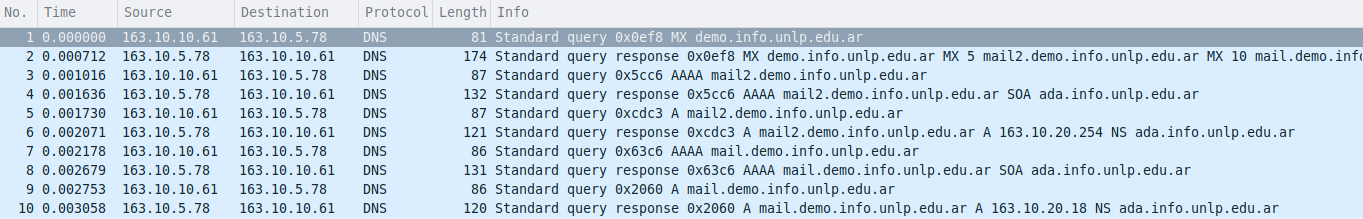
\includegraphics[width=1.0\textwidth]{dns}
    \caption{Consultas DNS realizadas por el servidor SMTP origen.}
\end{figure}

\begin{enumerate}[a)]
  \item ¿Cuál es el servidor DNS recursivo que utiliza el servidor SMTP origen? \\

  Mirando la primer consulta DNS realizada, podemos observar que el servidor DNS recursivo al cual hace la consulta tiene como IP 163.10.5.78. \\

  \item ¿Cuáles son las consultas DNS que realiza? \\

  Las consultas DNS realizadas son las siguientes:

  \begin{enumerate}[1.]
    \item Primero se hace una consulta DNS al servidor con IP 163.10.5.78 para obtener el servidor de mail de `demo.demo.info.unlp.edu.ar` haciendo una consulta DNS de tipo MX.

    En la respuesta de la misma se obtienen los datos de dos servidores de mail. Los mismos son `mail2.demo.info.unlp.edu.ar` y `mail.demo.info.unlp.edu.ar` con preferencias 5 y 10 respectivamente. \\

    \item Posteriormente, se pide conocer la IP del servidor de mail con mayor nivel de preferencia, 5. Entonces se hace una consulta DNS de tipo AAAA al mismo servidor que en el caso anterior para conocer la IPv6 del servidor de mail `mail2.demo.info.unlp.edu.ar`.

    Dado que la respuesta de la consulta es vacia y no existe ningun error en la conexión, podemos saber que el mismo no tiene una IPv6 asociada. \\

    \item Se procede a consultar por la IPv4 del servidor `mail2.demo.info.unlp.edu.ar` haciendo una consulta DNS de tipo A. En la respuesta de la consulta podemos ver que se obtiene la ip 163.10.20.254. \\

    \item Posteriormente, se pide conocer la IP del servidor de mail con nivel de preferencia 10. Entonces se hace una consulta DNS de tipo AAAA al mismo servidor que en el caso anterior para conocer la IPv6 del servidor de mail `mail.demo.info.unlp.edu.ar`.

    Dado que la respuesta de la consulta es vacia y no existe ningun error en la conexión, podemos saber que el mismo no tiene una IPv6 asociada. \\

    \item Se procede a consultar por la IPv4 del servidor `mail.demo.info.unlp.edu.ar` haciendo una consulta DNS de tipo A. En la respuesta de la consulta podemos ver que se obtiene la ip 163.10.20.18. \\
  \end{enumerate}

  \item ¿Alguna de las respuestas es de tipo autoritativa? \\

  Mirando el flag \textit{Authoritative} de las respuestas a cada una de las consultas podemos ver que ninguna de ellas son de tipo autoritativo. \\
\end{enumerate}

\section{Ejercicio 4}

Análisis de SMTP

\begin{enumerate}[a)]
  \item ¿A qué servidor SMTP se conecta el servidor de correo origen? ¿Por qué?

  Observando la primer fila de los datos correspondientes a SMTP podemos ver que el servidor de mail con el que se logra establecer la conexión tiene ipv4 163.10.20.18, es decir, que se conecta con el servidor `mail.demo.info.unlp.edu.ar`. \\

  \item ¿Cuántas comunicaciones SMTP se observan en la captura?

  Se observan dos comunicaciones SMTP. \\
\end{enumerate}

\section{Ejercicio 5}

Sobre el primer correo electrónico \\

\begin{enumerate}[a)]
  \item ¿A qué corresponde la información enviada por el servidor destino como respuesta al comando EHLO? Elija dos de las opciones del listado e investigue la funcionalidad de la misma.

  La información que envia el servidor como respuesta al EHLO es:

  \begin{itemize}
    \item mail
    \item PIPELINING
    \item SIZE 10240000
    \item VRFY
    \item ETRN
    \item STARTTLS
    \item AUTH PLAIN LOGIN
    \item AUTH=PLAIN LOGIN
    \item ENHANCEDSTATUSCODES
    \item 8BITTIME
    \item DSN
    \item SMTPUTF8
  \end{itemize}
  
  \textbf{STARTTLS}
  
  STARTTLS es una extensión a los protocolos de comunicación de texto plano, que ofrece una forma de mejorar desde una conexión de texto plano a una conexión cifrada (TLS o SSL) en lugar de utilizar un puerto diferente para la comunicación cifrada. \\
  
  \textbf{PIPELINING}
  
  La extensión pipelining significa que, durante la conexión, el cliente no siempre necesita esperar una respuesta antes de enviar la siguite solicitud. Especificamente, el cliente no necesita esperar por respuestas de RSET, MAIL, RCPT, o un mensaje codificado.
  
  El servidor puede demorar la respuesta mientras sigue recibiendo nuevas solicitudes, pero en general esto no ocurre. El servidor no debería nunca esperar por el input del cliente hasta haber terminado todas las solicitudes pendientes, y debe responderlas en order. Es responsabilidad del cliente evitar el deadlock. \\
  
  \textbf{SIZE}
  
  La extensión size tiene 2 propositos:
  
  \begin{itemize}
    \item Avisar al servidor de un estimado del tamaño del mensaje antes de que el mismo sea transmitido.
    \item Avisar el cliente de que los mensajes superando cierto tamaño no será aceptado. \\
  \end{itemize}

  \item ¿Por qué el contenido del primer mail no puede ser leído?

  Se envia el mail de forma segura utilizando TLS. \\
\end{enumerate}

\section{Ejercicio 6}

Con respecto al segundo correo electrónico

\begin{enumerate}[a)]
  \item ¿Cuál es el nombre del servidor de correo origen? \\

  El primer comando que necesitamos enviar al servidor de correo es EHLO o HELO. Este es un saludo básico que inicia la comunicación entre el cliente de telnet y el servidor SMTP. También se pasa el DNS PTR para la dirección IP desde la que nos conectamos, como se determinó previamente.

  Luego, el nombre del servidor de correo origen es `mail.linti.unlp.edu.ar` y lo sabemos dado que se envia como parámetro del comando EHLO. \\

  \item ¿Cuál es el MESSAGE-ID del correo enviado? ¿Quién asigna dicho valor?

  En la fila 20 de los datos filtrados para el protocolo SMTP, paquete nro. 113 del total de los paquetes del .pcap, se puede ver en el campo Internet Message Format el MESSAGE-ID del mail enviado y este es:
  
  \textit{$<$94c3492a-4bf1-c0c8-c059-c2cb2216d2f8@linti.unlp.edu.ar$>$}
  
  El Message-Id es generado por el user agent de mail o el servidor SMTP origin. \\
  
  \item ¿Cuál es el producto que implementa el servidor de correo origen y cuál el destino?
  
  El cliente utilizado para el envio del mail es Thunderbird, \textit{Mozilla/5.0 (X11; Linux x86\_64; rv:52.0) Gecko\/20100101 Thunderbird\/52.9.1}. Luego, el producto que implementa el servidor de correo origen es Exim en su versión 4.80, y el servidor de mail destino implementa Postfix sobre un GNU Debian. \\
  
  \item Analice y explique los comandos SMTP y las correspondientes respuestas que se presentan en la captura.
  
  \begin{itemize}
    \item EHLO, para abrir una sesión, en el caso de que el servidor soporte extensiones definidas en el RFC 1651.
    
    En ambos casos de utilización de este comando, el servidor responde con un listado de comandos extra soportados por el mismo. Entre estas opciones está PIPELINING la cual permite que se ejecuten los comandos MAIL FROM, RCPT TO y DATA sin esperar una respuesta del servidor inmediata entre cada uno de ellos. Se explican luego cada uno de los comandos. \\
    
    \item STARTTLS, Los servidores de correo electrónico y los clientes que usan el protocolo SMTP normalmente se comunican usando texto sin formato a través de Internet. La comunicación a menudo pasa por uno o más enrutadores que el servidor y el cliente no controlan ni confían en ellos. Esta comunicación se puede controlar y también es posible modificar los mensajes que se envían a través de los enrutadores. \\
    
    Para mejorar la seguridad, se puede usar una conexión encriptada TLS (Seguridad de la capa de transporte) al comunicarse entre el servidor de correo electrónico y el cliente. TLS es más útil cuando se necesita cifrar un nombre de usuario y contraseña de inicio de sesión (enviados por el comando AUTH). TLS se puede utilizar para encriptar todo el mensaje de correo electrónico, pero el comando no garantiza que todo el mensaje permanezca encriptado todo el camino hasta el receptor; algunos servidores de correo electrónico pueden decidir enviar el mensaje de correo electrónico sin cifrado. Pero al menos el nombre de usuario y la contraseña utilizados con el comando AUTH permanecerán encriptados. Usar el comando STARTTLS junto con el comando AUTH es una forma muy segura de autenticar usuarios. \\
    
    En respuesta a esto, el servidor envia 220 2.0.0 Ready to start TLS. \\
    
    \item MAIL FROM, para indicar quien envía el mensaje. \\
    
    \item RCPT TO, para indicar el destinatario del mensaje. \\
    
    \item DATA, para indicar el comienzo del mensaje, éste finalizará cuando haya una línea únicamente con un punto. \\
    
    \item QUIT, para cerrar la sesión. \\
    
    Como respuesta, el servidor envía 221 2.0.0 BYE. \\

  \end{itemize}
  
  En el caso de los comandos ejecutados para el envio de mail, como se menciona anteriormente se ejecuta en un pipe, y el servidor envia los tres códigos en una unica respuesta 250 2.1.0 Ok | 250 2.1.5 Ok | 354 End data with $<$CR$>$$<$LF$>$.$<$CR$>$$<$LF$>$. \\
  
  \item ¿Qué diferencia hay entre la entrada “MAIL FROM” y “From” que se observa en la captura?
  
  Para explicar la diferencia entre ambas podemos pensar en el siguiente ejemplo: 
  
  Cuando vos envía una carta, la envias en un sobre. El sobre contiene tu mensaje. La dirección de devolución escrita en el correo postal es la misma que la dirección de devolución "MAIL FROM:" y la "RCPT TO:" dará la dirección del destinatario. Esto es parte de la información del sobre.
  
  El contenido del mensaje, dentro del sobre de la carta, es como el cuerpo de su mensaje. En el sentido del correo electrónico, también puede tener la información del campo del encabezado, como "Subject:" "Date:", "To:" y "From:".

  Luego, el comando "MAIL FROM" especifica la dirección para propósitos de devolución (ejemplo: problemas con la entrega  de correo). Por otro lado, el campo de encabezado "De:" le dirá quién es el autor del mensaje. \\
  
  \item Indicar cuáles cabeceras fueron agregadas por el MUA.
  
  El MUA agrega las cabeceras de User Agent y Message ID. \\
  
  \item Analice las cabeceras MIME y responda:
  
  \begin{enumerate}[1)]
    \item ¿Qué tipo de archivo fue adjuntado al correo electrónico? 
    
    Se adjunta un archivo de tipo imagen con formato \textit{.jpeg}. \\
    
    \item ¿Quién es el personaje que se encuentra en la foto?
    
    \begin{figure}[H]
        \centering
        
\includegraphics[width=0.5\textwidth]{download.jpeg}
        \caption{Imagen enviada como archivo archivo adjunto en el mail.}
    \end{figure}
  \end{enumerate}
\end{enumerate}

\end{document}
